Beim Bau eines Schwimmbeckens oder ähnlichem wäre es sehr hilfreich für den 	Bauherren, wenn er Bescheid darüber wüsste, wie lange die anschliessende 		Befüllung des Beckens andauert. Oftmals kann man dies sehr schlecht 			abschätzen, weshalb es dann oft zu ungewollten Verzögerungen im 				Bauprojekt kommt. Daher haben wir es uns zur Aufgabe gemacht, eine 				Simulation mit MATLAB Simscape zu erstellen, die das Befüllen eines 			Wassertanks simuliert. Diese Simulation könnte dann auf verschiedene 			Bauprojekte von Wasserbecken angewandt werden.

%%%%%%%%%%%%%%%%%%%%%%%%%%%%%%%%%%%%%%%%%%%%%%%%%%%%%%%%%%%%%%%%%%%%%%%%%%%%%
\begin{figure}[htb]
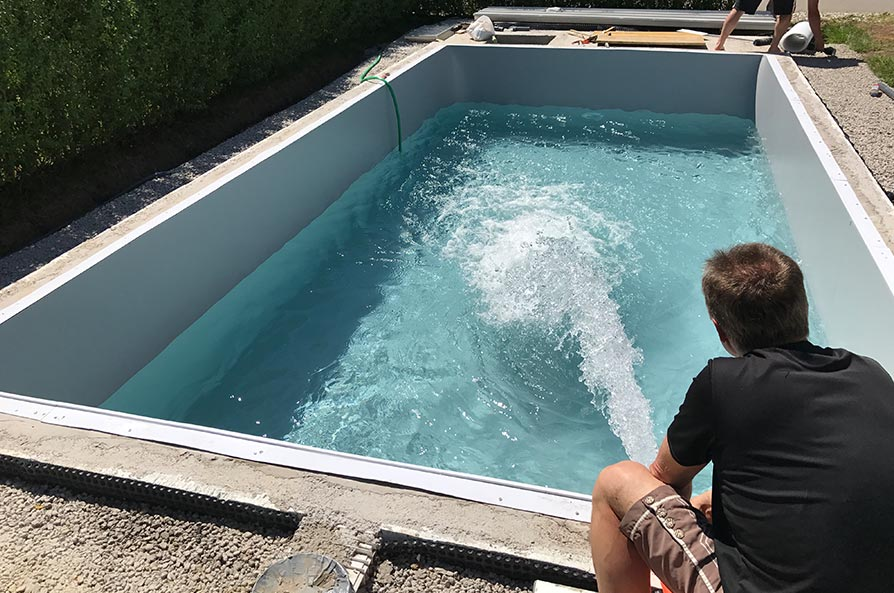
\includegraphics[width=\textwidth]{Sinnbild_Schwimmbecken.jpg}
\caption{Sinnbild zur Veranschaulichung einer Schwimmbeckenbefüllung}
\label{fig:Sinnbild zur Veranschaulichung einer Schwimmbeckenbefüllung}
\end{figure}
%%%%%%%%%%%%%%%%%%%%%%%%%%%%%%%%%%%%%%%%%%%%%%%%%%%%%%%%%%%%%%%%%%%%%%%%%%%%%

Ziel dieser Simulation soll sein, dass man durch diese Simulation einfach Abschätzen kann, was eine Wasserpumpe für einen Durchsatz liefert und wie lange eine Befüllung eines Wassertankes andauert. Dadurch sollen künftige Verzögerungen aufgrund von Fehleinschätzungen in Bauprojekten von 				Wasserbecken verhindert werden.